\documentclass[11pt]{article}
\usepackage[margin=1in]{geometry}
\usepackage{amsmath,amssymb,bm}
\usepackage{booktabs}
\usepackage{graphicx}
\usepackage{hyperref}
\usepackage{xcolor}
\usepackage{enumitem}
\hypersetup{colorlinks=true,linkcolor=blue!50!black,urlcolor=blue!50!black,citecolor=blue!50!black}
\graphicspath{{figures/}}
\newcommand{\sD}{s_D}
\newcommand{\sA}{s_A}
\newcommand{\tf}{t_f}
\newcommand{\code}[1]{\texttt{#1}}

\title{Building a Minimum-Time Costate Library over the Phase Torus:\\
Methods and Findings for the 70\,mN DRO\,$\to$\,Tulip Campaign}
\author{M. Casey, Coorbital Inc.}
\date{September 15, 2026}

\begin{document}
\maketitle

\begin{abstract}
A costate library keyed by departure and arrival phase is a $24\times24$
grid of minimum-time transfers, each a certified root of the Pontryagin
boundary-value problem. Filling every cell of the torus took eight rounds
over three days and, more importantly, five distinct families of
extremals that no single continuation could reach. This document explains
the techniques that built it -- the certification gate stack,
pseudo-arclength continuation in the arrival phase, the departure-phase
ribs, the family map, branch-blind direct solves for finding new families,
cell-by-cell direct filling, and the second-order sweep -- and what the
family shares reported in the campaign log mean. The operational recipe
is in \code{process/PHASE\_TORUS\_RUNBOOK.md}; the chronological record is
FINDINGS~\S59--72.
\end{abstract}

\section{The problem and the grid}

The transfer is the planar-symmetric CR3BP Earth--Moon low-thrust
minimum-time problem: a spacecraft of $m_0 = 150$\,kg with a 70\,mN, 900\,s
thruster leaves a distant retrograde orbit (period $\tau_D = 1.0$
nondimensional) and arrives on a 7-petal tulip orbit (branch $p = -1$,
period $\tau_A = 2\pi(N_p-2)/(N_p-1) = 5.236$). Both orbits are periodic,
so the boundary states are functions of a \emph{phase} in $[0,1)$: the
departure state is $\bm{x}_D(\sD)$ and the arrival state is
$\bm{x}_A(\sA)$. The pair $(\sD,\sA)$ lives on a torus, and the library is
the map $(\sD,\sA)\mapsto (\tf^\star,\bm{\lambda}(0))$ on the lattice
$\sD = k/24$, $\sA = 0.0754 + j/24$.

Each cell's entry is a root $z = (\bm{\lambda}(0), \tf)\in\mathbb{R}^8$
of the shooting equations of the PMP boundary-value problem: seven
costates at departure and the final time, such that the flown extremal
(bang control $\bm{u} = -\bm{\lambda}_v/|\bm{\lambda}_v|$ at full
throttle) lands on $\bm{x}_A(\sA)$ with the transversality condition
$\lambda_m(\tf) = 0$. Roots come in \emph{families} -- connected branches
in $(\sD,\sA,z)$ space -- and a given cell may lie under several of them;
the library keeps the fastest \emph{certified} one.

\section{What ``certified'' means: the gate stack}

Every entry in the library passed \code{certify\_root}, which does more
than converge the shooting equations:
\begin{enumerate}[nosep]
\item multiple-shooting residual on $K=24$ junctions below tolerance
  (\code{ms\_tfmin}, homogeneous chart; the polish is capped, so a stalled
  Newton cannot hang the campaign);
\item the flown arrival, re-integrated from $z$ alone with ode113 at
  $10^{-13}$, misses $\bm{x}_A(\sA)$ by less than a kilometre in position
  and by nothing measurable in velocity (``fly'');
\item transversality $\lambda_m(\tf)=0$ read off that tight flight (an
  earlier gate read it off an ode45 $10^{-10}$ flight and refused good
  roots -- FINDINGS~\S59);
\item the free-time conjugate test (Bonnard--Caillau--Tr\'elat, the
  quotiented Jacobi determinant sampled through $(0,\tf)$): no interior
  sign change, near-misses resolved by a dense scan;
\item the sufficiency-hypothesis gates: strong Legendre
  $\min_t|\bm{\lambda}_v| > 0$, $Q_{mt} > 0$, and normality with the
  abnormal-lift space of dimension one by a margin of at least $10\times$
  (``lift margin'');
\item lunar clearance of 1900\,km along the whole arc.
\end{enumerate}
A root that fails any gate is recorded with its reason and never enters
the catalog. This is what makes the availability grid honest: an empty
cell means \emph{no certified root found}, not \emph{not tried}.

\section{Pseudo-arclength continuation in the arrival phase}

The arrival axis is where the sensitivity lives -- the arrival state
moves along a long, highly curved tulip petal -- so it is walked by
pseudo-arclength continuation (\code{arclength\_ms},
\code{arclength\_arrival}) rather than a fixed-step walker. The unknowns
are the $K$ junction states plus $z$, augmented by a normality scalar
$\rho$ (the homogeneous chart of \code{ms\_tfmin\_hom}), and the
continuation parameter is $\sA$ (``$q$''). At each step the tangent of the
solution curve is computed from the Jacobian, a predictor step of length
$ds$ is taken along it, and a corrector Newton solve is done in the plane
orthogonal to the tangent; $ds$ adapts to the Newton count.

Three things the arc records are what the campaign lives on:
\begin{itemize}[nosep]
\item \textbf{crossings} of the grid levels: whenever $\sA$ passes a
  lattice value (possibly several times, unwrapped beyond $[0,1)$), the
  root is re-solved at exactly that level and stored -- these are the
  sheet's candidates;
\item \textbf{folds}: sign changes of the tangent's $\sA$-component,
  localised and classified (rank-one loss of $R_x$ with a regular
  augmented matrix) -- where the family turns back in arrival phase;
\item \textbf{the normality scalar} $\rho$ along the walk: $\rho\to 0$ is
  the family losing normality (the abnormal direction opening), a
  different kind of end from a fold.
\end{itemize}
An arc of 4000 steps is 2--6 hours of solves. Since 2026-09-15 the arc
so far is saved atomically every 50 steps (\code{.partialFile}), after a
MATLAB segfault at step 2160 of one walk left nothing on disk; the partial
is readable mid-walk and already answers ``which columns will this family
change''.

\section{The arrival sheet}

\code{sheet\_from\_arcs} assembles, per arrival phase, every candidate from
every arc's crossings and every seed (the library's own certified roots,
including the direct-found ones), certifies each, merges duplicates only
when both $\tf$ \emph{and} $z$ agree (keying on $\tf$ alone once merged
two distinct extremals), and takes the fastest certified candidate as the
column's \emph{spine}. Nothing is discarded: a column keeps all its
candidates with their verdicts, which is what lets the family map and the
gap analysis work later.

\section{Departure-phase ribs}

Departure phase enters the problem only through the first junction's
fixed state, so the departure axis is cheap: \code{rib\_from\_crossing}
holds $\sA$ and walks $\sD$ in steps of $1/24$ from the spine, re-solving
from the previous point's junctions and certifying every point; a failed
step is bisected up to eight times. A rib stops -- and says why -- when a
step cannot be certified even at $1/1728$ of a period: ``normal-chart
polish did not converge'' (the root leaves the chart's basin) or ``dense
conjugate scan not clear'' (a conjugate point is approaching). Every cell
beyond the stop is a hole for the direct filler.

Ribs run under a supervised work queue (\code{run\_costate\_library},
\code{campaign\_supervisor.sh}): one unit per column, process-held kernel
file locks, per-point checkpoints so a killed worker resumes mid-walk,
heartbeats per solve stage, a parent supervisor per worker, and a
finalizer that runs once when every column is published.

\section{Families and the family map}
\label{sec:families}

A \emph{family} is one connected branch of extremals. Operationally it is
named by its \emph{anchor} -- the certified root the arcs start from --
because the two arcs from an anchor (arrival phase increasing and
decreasing) trace that branch. \code{family\_map} reads, from the stored
arcs, each family's arrival-phase span, $\tf$ span, folds, normality
floor, and the \emph{kind} of each end of its span: a fold, the walk
budget (the branch continues, unmapped), a walk that ended with
$\rho\to0$, or the anchor itself (that direction never walked). It then
attaches every certified root at every column to the arc that passes
through it -- $\tf$ interpolated along the arc at that level, matched to
$10^{-5}$\,d; distinct roots at one phase sit $\ge 0.05$\,d apart -- and
every rib point to its spine root (the rib's first three points
extrapolated quadratically back to the spine). The catalog ships the map
as \code{cat\_.families} and an \code{int8} \code{family\_index} per entry.

This is the meaning of the sentence in the campaign log, ``\emph{Five
families now share the torus: fast 47\%, direct18 22\%, fast2 13\%,
direct11 13\%, plus 24 cells on roots no arc has walked}'' (round 6; the
final numbers are in Table~\ref{tab:families}):
\begin{itemize}[nosep]
\item the percentages are shares of the certified cells attributed to
  each family through the rib that produced them -- 47\% of the cells lie
  on ribs walked off spines of the original family;
\item \code{family\_index} $= -1$, ``roots no arc has walked'': certified
  spine roots at $\sD=0$ that no arc passes through -- the direct solver
  found them and no continuation has been anchored on them. Each is a
  candidate anchor; the direct18 and direct11 families were exactly such
  roots before their arcs were walked;
\item \code{family\_index} $= -2$: rib points whose spine root the map
  could not identify -- ribs from an earlier round whose spine is not
  among this sheet's roots, and the direct-solved cells, which have no
  spine at all.
\end{itemize}

\begin{table}[h]\centering
\caption{The families of the finished torus (round 8). Spans are in
arrival phase, unwrapped; ``$\tf$'' is the family's range at $\sD=0$.}
\label{tab:families}
\begin{tabular}{llllll}
\toprule
family & anchor ($\sA$, $\tf$) & span & $\tf$ (d) & ends & cells \\
\midrule
fast & 0.0754, 17.80\,d & 0.034--0.841 & 16.2--25.7 & fold / fold & 242 (42\%) \\
A2 & 0.9087, 26.43\,d & 0.908--1.711 & 26.0--44.1 & fold / budget & 0 \\
fast2 & 0.8671, 17.25\,d & 0.800--1.394 & 16.9--25.3 & fold (S-bend) / fold & 72 (12.5\%) \\
direct18 & 0.7837, 17.83\,d & 0.573--1.224 & 16.8--38.2 & fold / fold & 121 (21\%) \\
direct11 & 0.4921, 17.96\,d & 0.357--0.715 & 17.8--32.4 & fold / stall & 69 (12\%) \\
\midrule
\multicolumn{5}{l}{roots no arc has walked ($-1$)} & 22 (3.8\%) \\
\multicolumn{5}{l}{rib points without an identified spine ($-2$)} & 50 (8.7\%) \\
\bottomrule
\end{tabular}
\end{table}

\section{Finding families the continuation cannot reach}
\label{sec:discovery}

The central lesson of the campaign. Continuation follows its own sheet:
from the original family's anchor the arcs reached $\sA = 0.841$ and
folded back, and the A2 family found at 0.9087 was 26\,d -- so the first
library reported 19 of 24 arrival phases and 22--26\,d transfers on
0.6--0.9, all certified minima of \emph{their} branches. The fast roots
were found by \emph{branch-blind direct solves}: a Hermite--Simpson
collocation solve with Sundman regularisation (\code{casadi\_mintime\_dro},
$N=800$, lunar clearance as a path constraint) at the phase in question,
warm-started from the \emph{other} family's certified flight; the
collocation solver does not know which branch it started on and lands in
the basin of the fastest nearby extremal. Its solution is harvested into
a multiple-shooting seed (\code{harvest\_ms\_seed}: covectors from the
defect multipliers, sign vote) and certified by the same gate stack. That
found 17--19\,d roots across 0.78--1.03 (seven days under the sheet), then
0.4921 at 17.96\,d (2.3 days under the sheet). Each became an anchor, its
arcs were walked, the sheet was rebuilt with the new crossings, and the
family map attributed every column.

A refused direct result is information too: at 0.5754 the fastest thing
the solver finds rides the 1900\,km clearance floor -- a constrained arc,
not an unconstrained extremal -- so the 21.45\,d root stands there.

\section{Cell-by-cell direct filling and the improve pass}

After the ribs, 38 cells were still empty. \code{fill\_holes\_direct}
solves each hole directly, warm-started from up to three certified
neighbours -- the same column's first, because they share the arrival
geometry (a rib \emph{is} this continuation), then the same row's --
harvests, certifies, keeps the fastest certified root and makes it a seed
for the cells still to come, so a column chains like a rib. All 38
certified. Two lessons: a neighbouring-column seed at a different
arrival phase sends the collocation solver to 100--400\,d junk (cap the
solve at 300\,s; try the column first), and run under R2026a (the
Parallel Computing Toolbox is not licensed under R2025b, and
certification needs the pool).

The \emph{improve pass} applies the same solve to filled cells more than
2\,d slower than a column neighbour, seeded from faster neighbours only,
keeping a root only if faster, and queueing the next slower neighbour
when a cell improves. Column 15 ($\sA=0.6587$), where the direct18 rib had
stalled at once and the fast family's 22--25\,d rib filled the column,
came down to 17.1--17.8\,d over nine cells; nine cells above $\sD=0.54$
resisted from both sides -- a fold of the direct18 sheet in the departure
phase, probably -- and keep the 23\,d family.

\section{The second-order sweep and its sidecar}

Every packaged entry is re-measured by \code{second\_order\_pass}: the
conjugate determinant densely through $(0,\tf)$ (interior crossings,
near-misses, multiplicity), the H6 margin $\lambda_m(0) < c/T$, the lift
margin. The measurements are written back into the catalog and kept in a
resumable \emph{sidecar} keyed by cell and $z$; when a catalog is
re-packaged with more ribs the sidecar is merged -- a record reused only
for the entry whose cell and $z$ match, everything else measured fresh --
so a re-packaging costs only the changed entries.

\section{The campaign loop and its monitoring}

A round is: sheet from every arc and seed $\to$ ribs for the columns
whose spine changed $\to$ package with every round's ribs offered (the
fastest certified point per cell wins) $\to$ audit (every entry re-flown
and re-gated) $\to$ sweep. A new round starts whenever a new family
changes spines (Section~\ref{sec:discovery}); a re-package without
walking follows the direct filler. Eight rounds took the library from 406
entries and 19 columns to 576 of 576 (Table~\ref{tab:rounds}).

Long jobs write their product after every item (arcs: partial saves;
ribs: per-point checkpoints; filler: per cell; sweep: per chunk), log to
files (batch MATLAB buffers stdout), and are watched by scripts that exit
on the job's DONE line, its death, an error, a silent log or an hourly
tick. A job at 0\,\% CPU after its banner is diagnosed through its
\code{matlab\_helper} child -- on 2026-09-15 a \code{git rev-parse} inside
\code{system()} hung on the Xcode licence prompt for an hour; the chain
now reads \code{.git} itself and trusts a process count only when it is
made of integers.

\begin{table}[h]\centering\small
\caption{The rounds.}
\label{tab:rounds}
\begin{tabular}{lp{0.62\textwidth}l}
\toprule
round & what changed & entries / verdict \\
\midrule
1 & first $24\times24$ from the original family & 406, 19 columns \\
2 & corrected transversality gate, supervised queue & 409, audit 409/0 \\
3 & fast2 anchor and direct roots seeded & 432 \\
4 & sheet from all six arcs and exact-phase seeds: 24/24 columns & 515, audit 515/0 \\
5 & direct18 arcs: columns 14--17, 20 take 16.8--19.0\,d & 534, audit 534/0 \\
6 & direct11 arcs: columns 11--13 take 18.0--18.8\,d & 538, audit 538/0 \\
7 & + \code{fill\_holes\_direct}, 38/38 & 576, audit 576/0 \\
8 & + improve pass, merged sidecar & 576/576, audit 576/0, sweep clean \\
\bottomrule
\end{tabular}
\end{table}

\section{Results}

The finished library (Figure~\ref{fig:torus}): 576 of 576 cells, $\tf$
from 16.23 to 23.86\,d (median 18.42\,d); audit 576 ok / 0 bad; sweep
576 done with 0 interior conjugate crossings, worst H6 margin $4.44\times$,
worst lift margin $10.6\times$. Every column is within 2.5\,d of its own
minimum except the nine stuck cells of column 15.

\begin{figure}[h]\centering
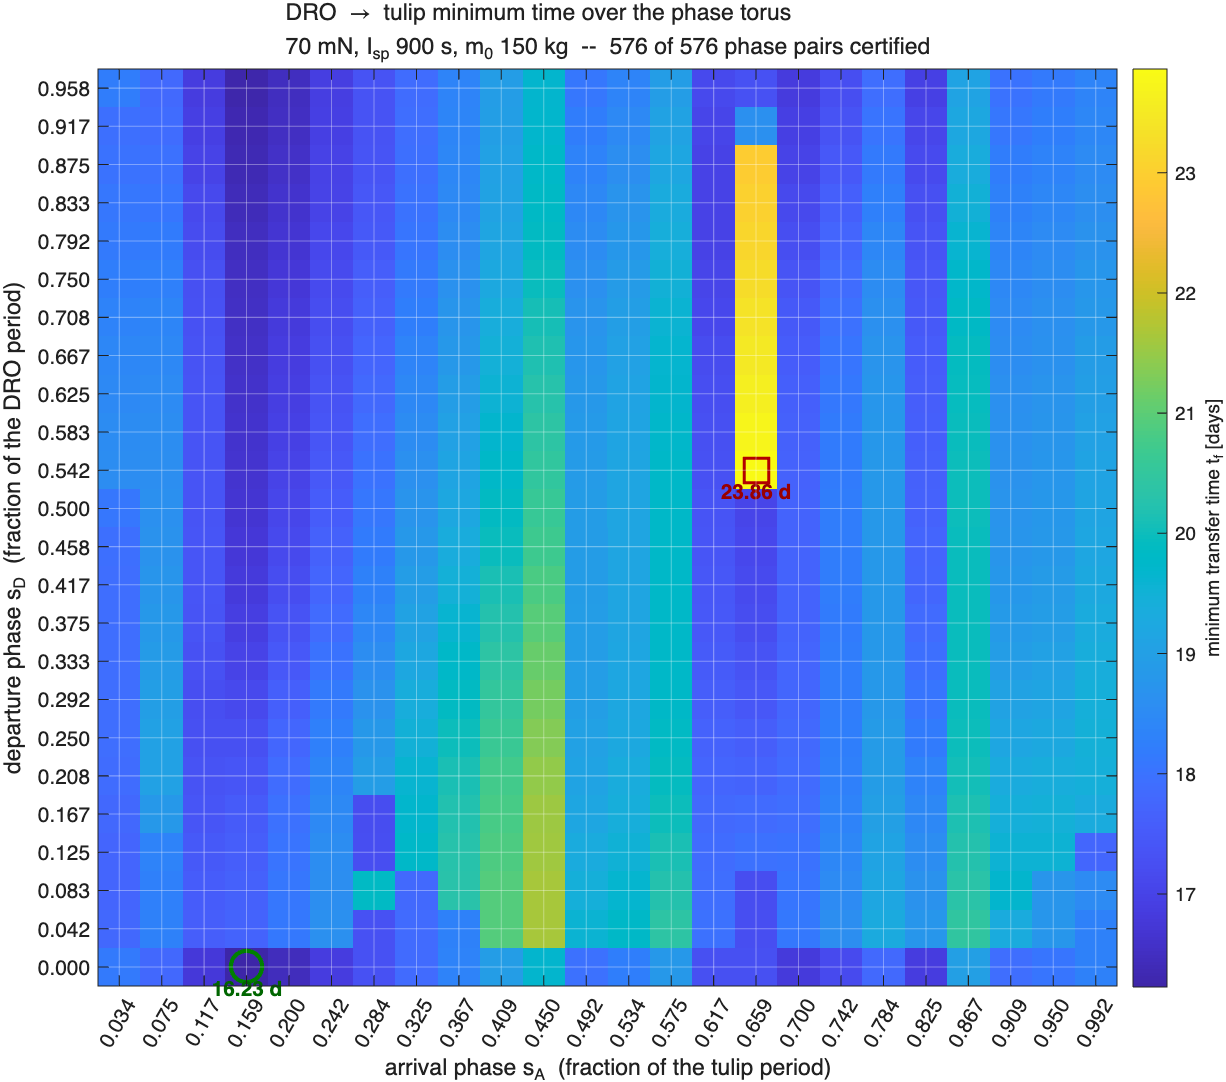
\includegraphics[width=0.85\textwidth]{phase_torus_70mN_24x24}
\caption{The phase torus: minimum time (days) over departure phase
(rows) and arrival phase (columns), round 8. The ridge along
$\sA\approx0.45$ is the original family's slow end; the plateau above
$\sA = 0.6$ is the direct18 and fast2 families; column 15's upper cells
are the 23\,d family the improve pass could not displace.}
\label{fig:torus}
\end{figure}

\paragraph{Open questions.} (i) Whether the nine column-15 cells are true
minima at 23\,d or a fold the direct solver cannot jump -- an arc in $\sD$
at $\sA=0.6587$ would say. (ii) The 22 spine roots no arc has walked
(0.9921 at 18.30\,d, 0.0337 at 18.14\,d among them): arcs from them would
attribute the last unmapped entries and might expose a sixth family.
(iii) The fast sheet is not one branch: below the direct18 fold at 0.59
the direct11 family carries 0.49--0.60, and between them the cell at
0.5754 is clearance-limited; the topology of the fast sheet as a whole --
how the five branches connect through their folds -- is not yet drawn.

\end{document}
